\usepackage[utf8]{inputenc}
\usepackage{graphicx}
\usepackage{placeins}
\usepackage{float}
\usepackage{titlepic}
\usepackage[T1]{fontenc}
\usepackage{babel}
\usepackage[export]{adjustbox} % sets maxwidth/maxheight for pictures
\usepackage{lipsum}
\usepackage{wrapfig} % wrap text around figures

\usepackage{titlesec}

\titleformat{\section}
  {\normalfont\Large\bfseries}{\thesection}{1em}{}[{\titlerule[0.8pt]}]
\titleformat{\subsection}
  {\normalfont\Large\bfseries}{\thesection}{1em}{}[{\titlerule[0.5pt]}]

%%% Picture on the side, before paragraph
%\begin{wrapfigure}[INSERT AMOUNT OF ROWS HERE]{r}{0.5\linewidth}
%\centering
%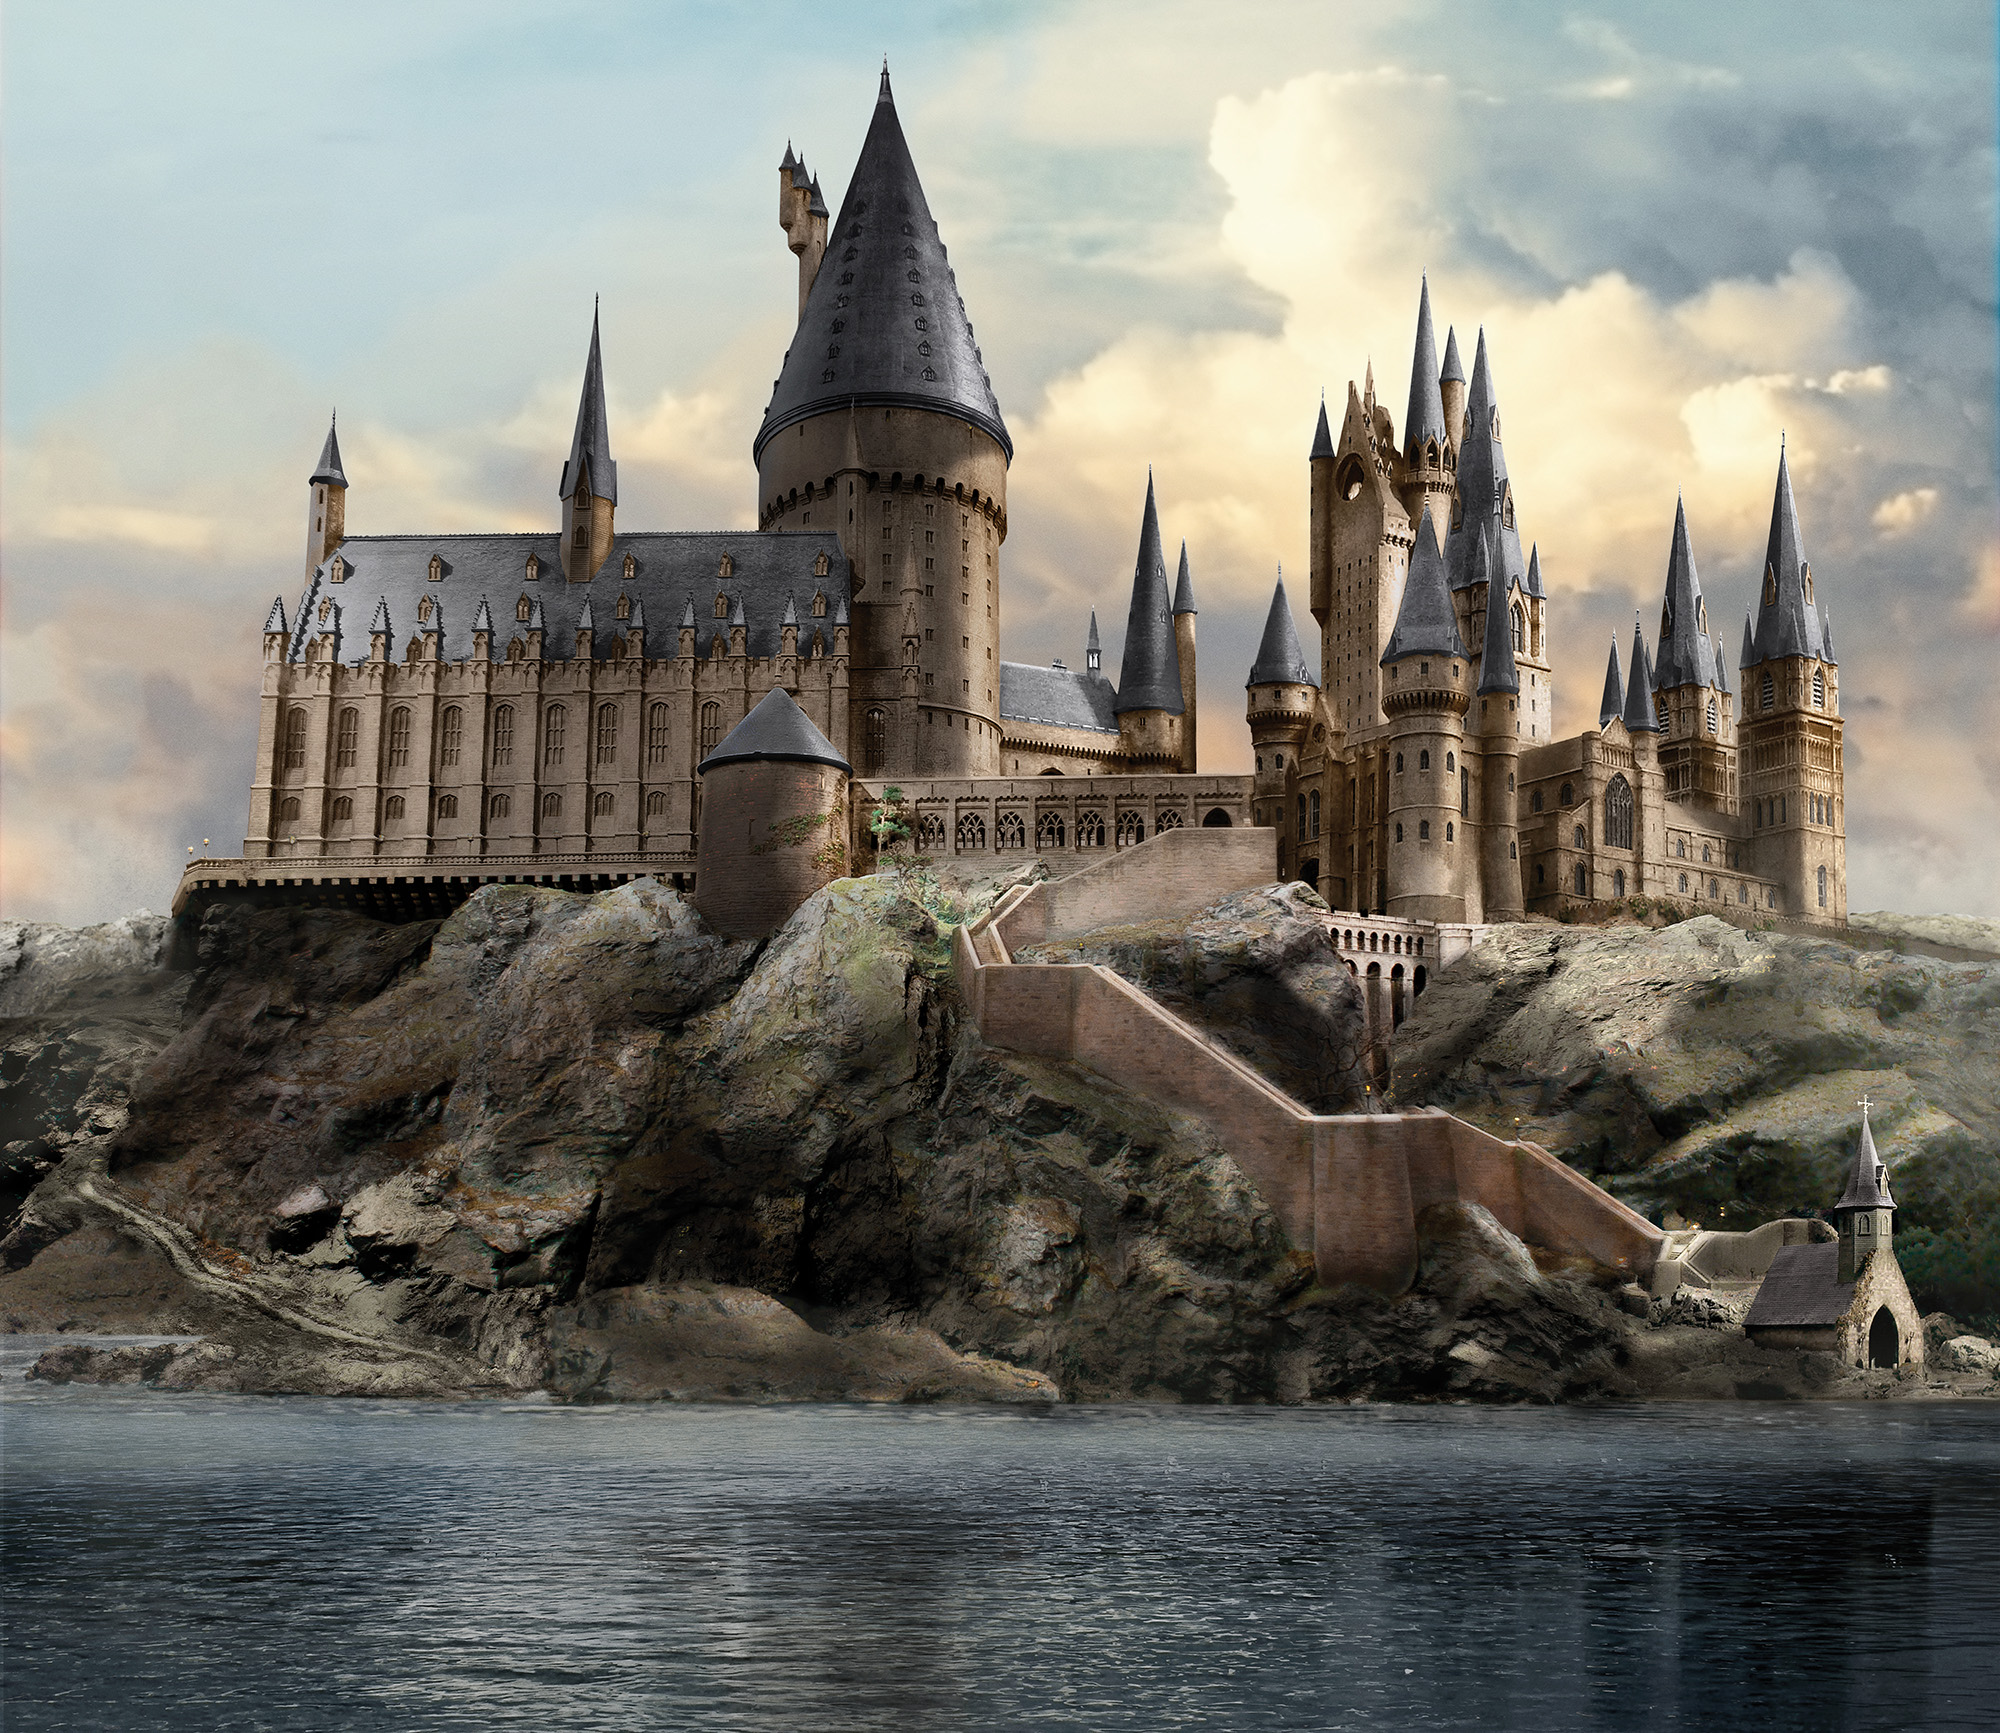
\includegraphics{../Pictures/Locations/Hogwarts/Castle_picture.png} 
%\caption{Hogwarts Castle}
%\end{wrapfigure}

%%% Picture full page width, after paragraph
%\begin{figure}[H]
%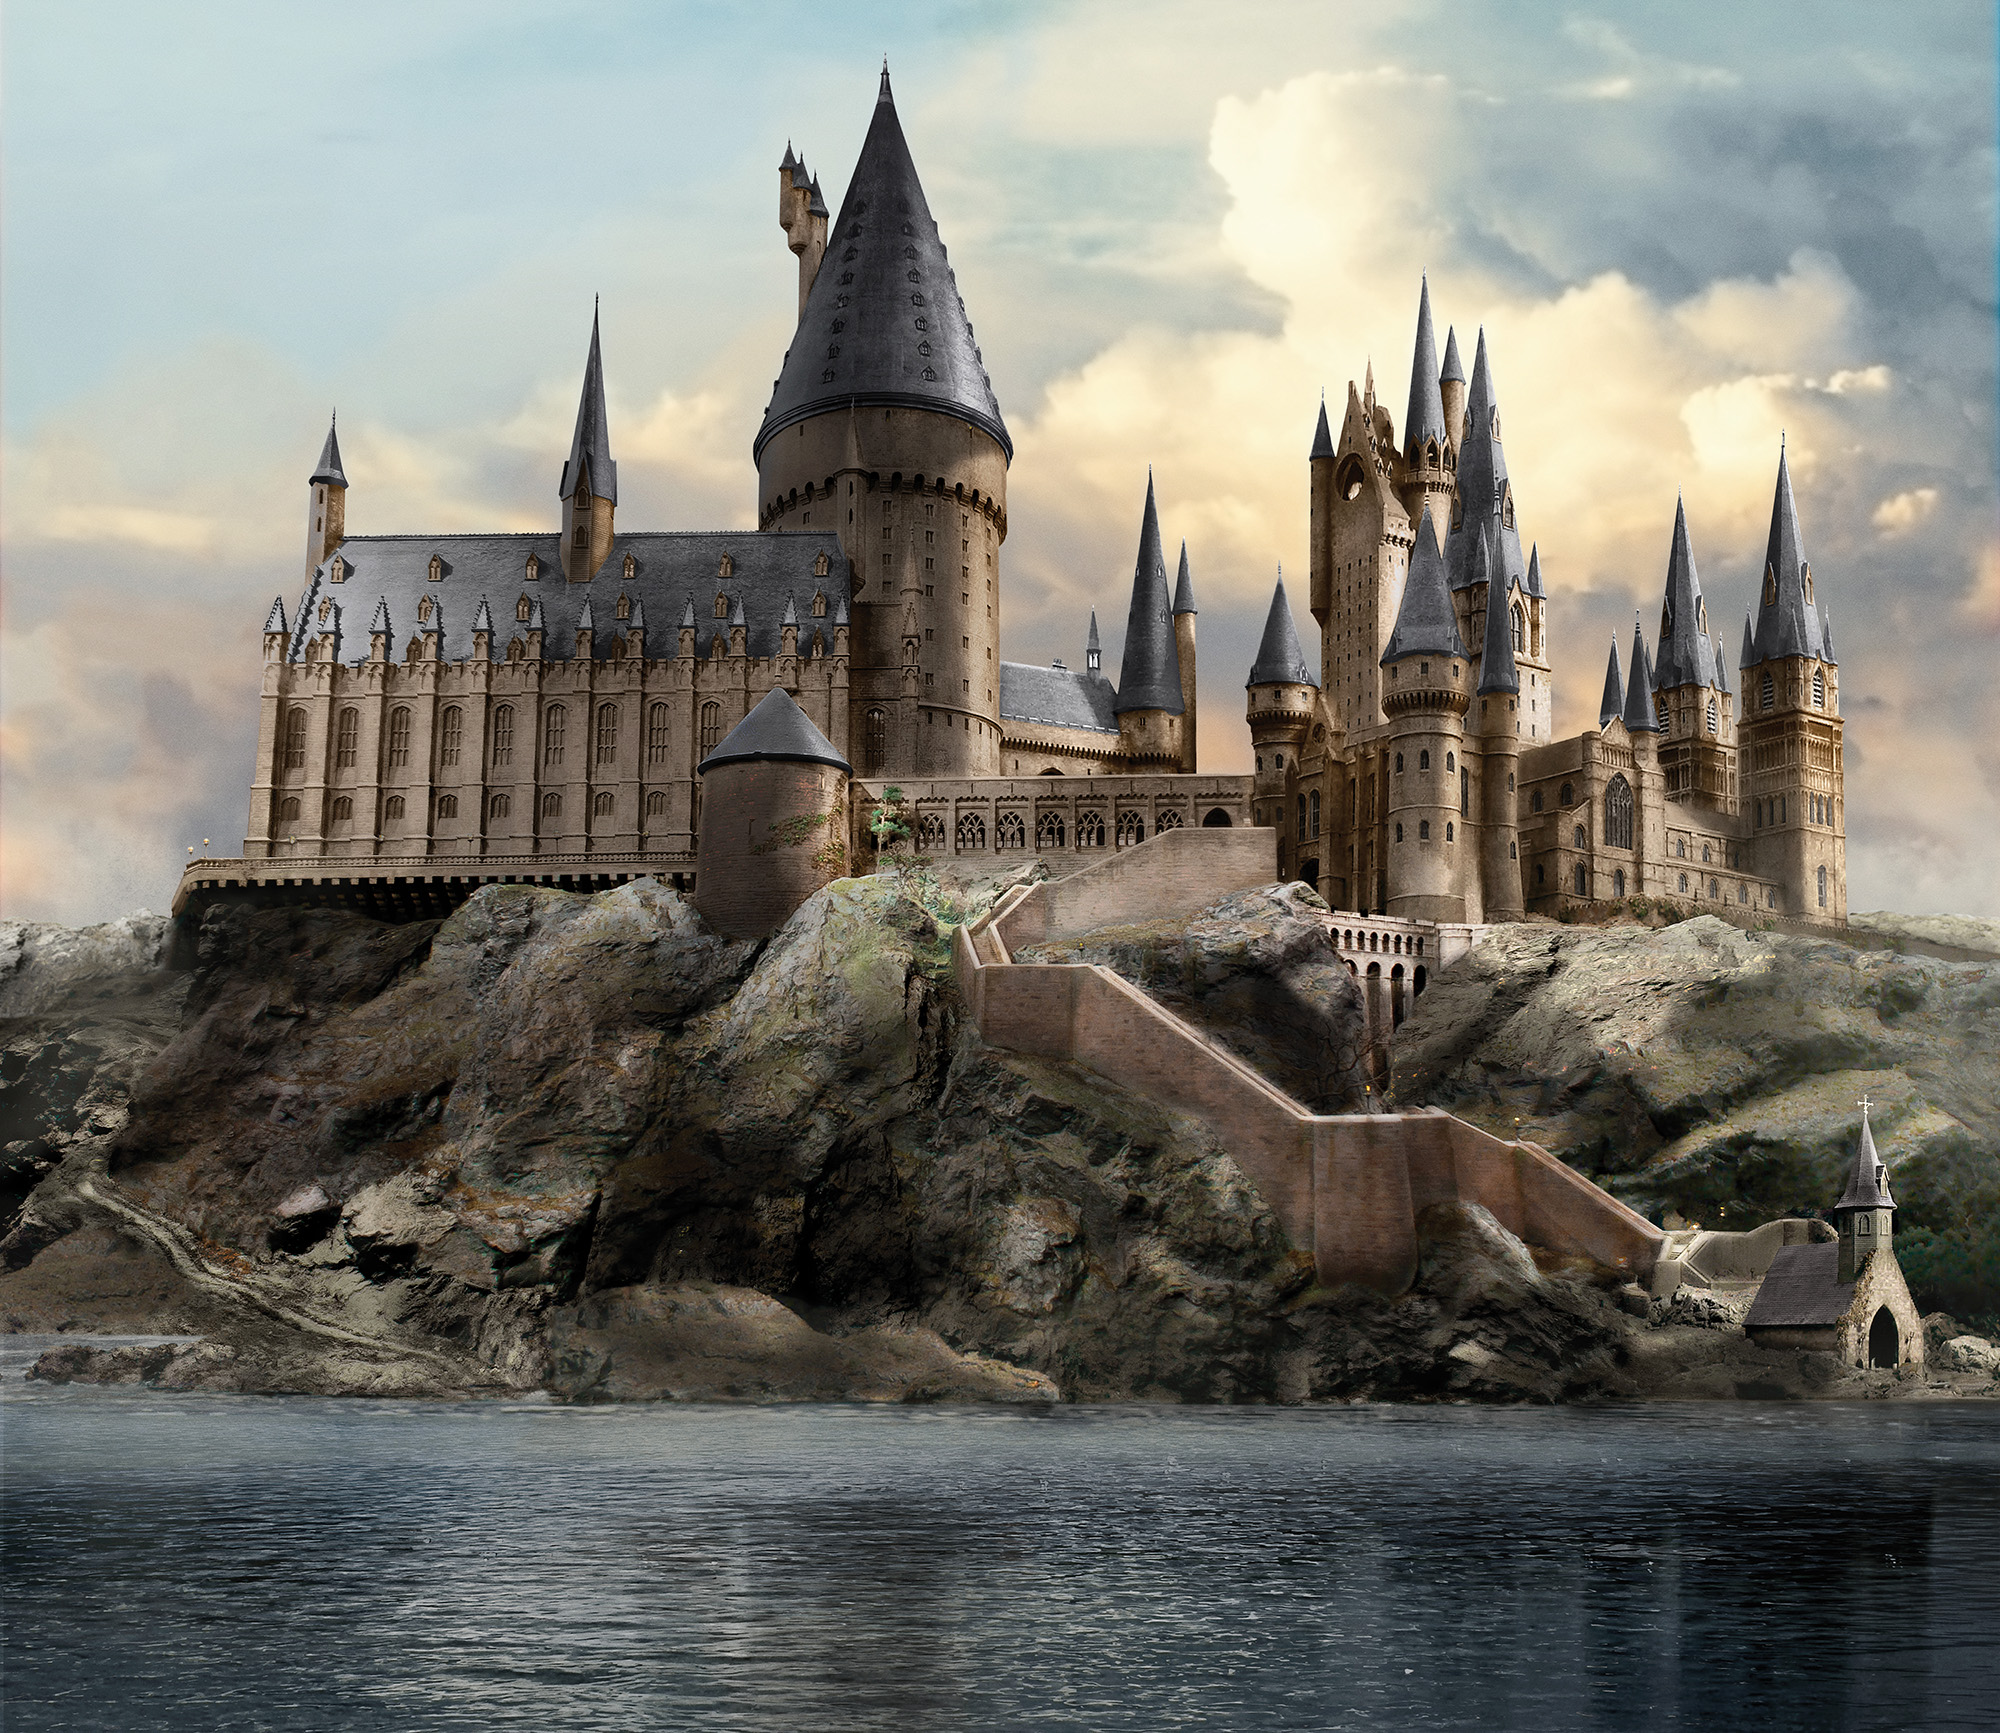
\includegraphics[\textwidth]{../Pictures/Locations/Hogwarts/Castle_picture.png} 
%\end{figure}